%% ═══════════════════════════════════════════════════════════════════════════════
%% CHAPITRE 1 — Contexte général, problématique et état de l'art
%% ═══════════════════════════════════════════════════════════════════════════════

\chapter{Contexte g\'en\'eral, probl\'ematique et \'etat de l'art}

%%──────────────────────────────────────────────────────────────────────────────
\section{Introduction du chapitre}
%%──────────────────────────────────────────────────────────────────────────────

La g\'en\'eralisation des technologies num\'eriques dans l'enseignement sup\'erieur constitue aujourd'hui l'un des leviers strat\'egiques les plus significatifs pour l'am\'elioration de la qualit\'e p\'edagogique, la continuit\'e des activit\'es acad\'emiques et l'inclusion \'educative. Dans ce contexte de mutation profonde, les \'etablissements universitaires sont confront\'es \`a un imp\'eratif d'adaptation organisationnelle et technologique, auquel r\'epondent des environnements num\'eriques de plus en plus sophistiqu\'es~\cite{unesco_digital_2026,worldbank_edtech_2026}.

Le pr\'esent chapitre constitue le socle analytique et conceptuel du projet \textbf{EduConnect}. Il poursuit quatre objectifs compl\'ementaires~: (i)~d\'ecrire le contexte mondial et national de la transformation num\'erique de l'enseignement~; (ii)~formuler la probl\'ematique ayant motiv\'e la conception d'EduConnect~; (iii)~pr\'esenter les objectifs et la m\'ethodologie adopt\'es~; et (iv)~dresser un \'etat de l'art approfondi des solutions existantes, afin de positionner EduConnect par rapport aux r\'ef\'erences du domaine.

Ce chapitre est organis\'e comme suit~: la section~\ref{sec:contexte} traite du contexte g\'en\'eral~; la section~\ref{sec:problematique} formule la probl\'ematique~; la section~\ref{sec:objectifs} d\'etaille les objectifs~; la section~\ref{sec:methodo} pr\'esente la d\'emarche m\'ethodologique~; la section~\ref{sec:etat_art} constitue l'\'etat de l'art~; la section~\ref{sec:positionnement} positionne EduConnect~; la section~\ref{sec:figures} pr\'esente les figures requises~; enfin, la section~\ref{sec:conclusion} conclut le chapitre.

%%──────────────────────────────────────────────────────────────────────────────
\section{Contexte g\'en\'eral}
\label{sec:contexte}
%%──────────────────────────────────────────────────────────────────────────────

\subsection{Transformation num\'erique de l'enseignement sup\'erieur \`a l'\'echelle mondiale}

La transformation num\'erique de l'\'education s'est acc\'el\'er\'ee de mani\`ere consid\'erable au cours de la derni\`ere d\'ecennie, port\'ee par la g\'en\'eralisation de l'acc\`es \`a Internet, la mont\'ee en puissance des technologies mobiles et, plus r\'ecemment, l'\'emergence de l'intelligence artificielle appliqu\'ee aux processus p\'edagogiques. L'Union internationale des t\'el\'ecommunications (UIT) indique que 6~milliards de personnes, soit environ 74\,\% de la population mondiale, utilisaient Internet en 2025, tout en soulignant que 2,2~milliards d'individus demeurent exclus de cet acc\`es, principalement dans les pays \`a revenus faibles et interm\'ediaires~\cite{itu_facts_2025}.

L'UNESCO confirme que si la connectivit\'e progresse \`a l'\'echelle mondiale, elle reste profond\'ement in\'egale~: seulement 40\,\% des \'ecoles primaires et 50\,\% des \'etablissements du secondaire inf\'erieur sont connect\'es \`a Internet dans le monde~\cite{unesco_gem_2023}. Ces donn\'ees soul\`event des questions fondamentales de politique \'educative et d'\'equit\'e d'acc\`es aux ressources num\'eriques, que l'UNESCO aborde dans ses cadres de comp\'etences num\'eriques et ses recommandations sur les ressources \'educatives libres~\cite{unesco_oer_2019,unesco_digital_2026}.

La Banque mondiale souligne que l'EdTech repr\'esente une opportunit\'e in\'edite pour les pays \`a revenus interm\'ediaires~: si elle est soutenue par des comp\'etences num\'eriques fondamentales et une connectivit\'e ad\'equate, elle peut contribuer \`a r\'eduire la crise d'apprentissage mondiale, notamment dans les communaut\'es souffrant de p\'enurie d'enseignants~\cite{worldbank_edtech_2026}. Toutefois, cette m\^eme institution met en garde contre les risques li\'es \`a la s\'ecurit\'e des donn\'ees et le risque d'aggravation des in\'egalit\'es \'educatives en l'absence de politiques d'encadrement adapt\'ees.

\subsection{Contexte national et enjeux institutionnels}

Dans le contexte alg\'erien et plus particuli\`erement au sein des universit\'es telles que l'Universit\'e des Sciences et de la Technologie d'Oran Mohamed~Boudiaf (USTO-MB), la gestion des activit\'es p\'edagogiques souffre d'une fragmentation des outils et des canaux de diffusion. Les ressources sont souvent partag\'ees via des messageries instantan\'ees non structur\'ees, les annonces ne parviennent pas syst\'ematiquement aux \'etudiants concern\'es, et les enseignants manquent d'un espace centralis\'e pour organiser leurs productions p\'edagogiques par module et par niveau d'\'etudes.

Ce constat est confirm\'e par les travaux r\'ecents r\'ealis\'es dans notre d\'epartement~: le m\'emoire portant sur une biblioth\`eque virtuelle de partage de livres~\cite{memoire_bibliotheque_2025} d\'eploie une solution web pour la diffusion de ressources textuelles~; le m\'emoire consacr\'e \`a une application mobile de branding~\cite{memoire_branding_2025} met en \'evidence l'importance d'une architecture orient\'ee utilisateur et d'une exp\'erience mobile soign\'ee~; enfin, le m\'emoire sur l'agriculture durable~\cite{memoire_agriculture_2024} illustre la maturit\'e des outils num\'eriques comme vecteurs de valorisation des connaissances scientifiques. Ces trois travaux partagent une structure acad\'emique convergente en quatre parties~: contexte/besoins, conception UML, impl\'ementation, \'evaluation~; c'est cette structure que le pr\'esent m\'emoire adopte et enrichit.

%%──────────────────────────────────────────────────────────────────────────────
\section{Probl\'ematique}
\label{sec:problematique}
%%──────────────────────────────────────────────────────────────────────────────

La gestion des activit\'es p\'edagogiques dans un contexte universitaire contemporain fait face \`a un d\'efi central~: la multiplicit\'e des outils et des canaux de communication g\'en\`ere une dispersion informationnelle qui nuit \`a la coh\'erence de l'exp\'erience acad\'emique. Les ressources p\'edagogiques~--- cours, travaux dirig\'es, travaux pratiques, examens, corrig\'es et supports multim\'edias~--- sont dispers\'ees sur des supports h\'et\'erog\`enes, sans structuration par module ni tra\c{c}abilit\'e des mises \`a jour.

Par ailleurs, la communication entre enseignants, mod\'erateurs et \'etudiants s'appuie souvent sur des outils grand public non con\c{c}us pour les usages acad\'emiques, ce qui engendre des probl\`emes de s\'ecurit\'e, de gouvernance et de qualit\'e de service. L'absence d'un syst\`eme de notification centralis\'e, d'un espace de publication structur\'e et d'un planificateur int\'egr\'e contraint les acteurs \`a recourir \`a des solutions de contournement chronophages et peu fiables.

\medskip
\noindent\fcolorbox{ustoblue}{ustolightblue!20}{\parbox{0.96\textwidth}{%
\textbf{Question de recherche~:} Comment concevoir et d\'evelopper une plateforme num\'erique unifi\'ee, s\'ecuris\'ee et modulaire, capable de centraliser les ressources p\'edagogiques, de faciliter la communication entre les diff\'erents acteurs de la communaut\'e acad\'emique, et de soutenir l'organisation du travail collectif, tout en restant accessible, maintenable et adapt\'ee au contexte universitaire local\,?
}}
\medskip

%%──────────────────────────────────────────────────────────────────────────────
\section{Objectifs du projet}
\label{sec:objectifs}
%%──────────────────────────────────────────────────────────────────────────────

\subsection{Objectif g\'en\'eral}

L'objectif g\'en\'eral du projet est de concevoir, d\'evelopper et valider \textbf{EduConnect}~: une plateforme web de partage p\'edagogique et de collaboration acad\'emique, con\c{c}ue pour les usages universitaires et structur\'ee autour d'une architecture orient\'ee modules, d'un syst\`eme de gouvernance par r\^oles et d'une couche sociale int\'egr\'ee.

\subsection{Objectifs sp\'ecifiques}

\begin{itemize}
  \item[\textbf{OS1.}] Centraliser les ressources p\'edagogiques (cours, TD, TP, examens, corrig\'es, playlists) dans une architecture hi\'erarchique~: Niveau $\rightarrow$ Module $\rightarrow$ Section $\rightarrow$ Ressource.
  \item[\textbf{OS2.}] Mettre en \oe uvre un syst\`eme d'authentification s\'ecuris\'e par jetons JWT et une autorisation par r\^oles~: Administrateur global, Mod\'erateur et Utilisateur.
  \item[\textbf{OS3.}] Int\'egrer un espace de communication structur\'e~: publications, commentaires, votes, partages et messagerie instantan\'ee (chat priv\'e et de groupe).
  \item[\textbf{OS4.}] D\'evelopper un syst\`eme de notifications permettant le suivi des \'ev\'enements acad\'emiques avec compteur de non-lus.
  \item[\textbf{OS5.}] Proposer un planificateur hebdomadaire pour la gestion collective des activit\'es et des \'ech\'eances.
  \item[\textbf{OS6.}] Garantir la tra\c{c}abilit\'e compl\`ete des actions de gestion~: ajout, modification et suppression des ressources, contr\^ol\'ees par le syst\`eme de r\^oles.
\end{itemize}

%%──────────────────────────────────────────────────────────────────────────────
\section{D\'emarche m\'ethodologique}
\label{sec:methodo}
%%──────────────────────────────────────────────────────────────────────────────

La d\'emarche adopt\'ee suit un processus incr\'emental en cinq phases, conforme aux pratiques reconnues en ing\'enierie des syst\`emes d'information et aux recommandations des travaux de r\'ef\'erence analys\'es~:

\begin{enumerate}
  \item \textbf{Analyse des besoins}~: identification des besoins fonctionnels et non fonctionnels par l'\'etude des usages existants, l'analyse de la litt\'erature et la consultation des trois m\'emoires de r\'ef\'erence.
  \item \textbf{Mod\'elisation conceptuelle}~: repr\'esentation des interactions par des diagrammes UML (cas d'utilisation, s\'equence, classes) pour formaliser les sc\'enarios et l'architecture logique.
  \item \textbf{Conception de l'architecture}~: d\'efinition de l'architecture applicative (API REST, frontend SPA) et du sch\'ema de la base de donn\'ees relationnelle PostgreSQL.
  \item \textbf{Impl\'ementation et int\'egration}~: d\'eveloppement progressif par fonctionnalit\'es (authentification, ressources, social, notifications, planificateur, administration), avec validation continue.
  \item \textbf{Tests et ajustements}~: validation fonctionnelle, tests de s\'ecurit\'e et ajustements selon les retours d'exp\'erience.
\end{enumerate}

%%──────────────────────────────────────────────────────────────────────────────
\section{\'Etat de l'art}
\label{sec:etat_art}
%%──────────────────────────────────────────────────────────────────────────────

\subsection{D\'efinitions et concepts cl\'es}

\paragraph{Syst\`eme de gestion de l'apprentissage (LMS).}
Un LMS (\textit{Learning Management System}) est un logiciel permettant de cr\'eer, distribuer et g\'erer du contenu p\'edagogique, ainsi que de suivre la progression des apprenants~\cite{moodle_overview_2026}. Les principaux LMS du march\'e incluent Moodle, Canvas et Blackboard.

\paragraph{Plateforme collaborative.}
Une plateforme collaborative est un environnement num\'erique qui offre des fonctionnalit\'es de communication, de co-production et de gestion des activit\'es pour des groupes d'utilisateurs. Elle peut int\'egrer des outils de messagerie, de partage de fichiers, de planification et de gestion de projets.

\paragraph{Apprentissage en ligne (\textit{e-learning}).}
L'e-learning d\'esigne l'ensemble des modalit\'es d'enseignement et d'apprentissage faisant appel aux technologies num\'eriques, qu'elles soient synchrones (classes virtuelles, visioconf\'erence) ou asynchrones (cours en ligne, forums, documents partag\'es)~\cite{unesco_digital_2026}.

\subsection{Pr\'esentation des solutions de r\'ef\'erence}

\paragraph{Moodle.}
Moodle est l'un des LMS open source les plus utilis\'es dans le monde. Il offre une gestion fine des cours, des activit\'es et des \'evaluations, ainsi qu'un syst\`eme d'extensions (plugins) permettant une forte personnalisation. Sa gouvernance institutionnelle est tr\`es flexible, mais son d\'eploiement exige des comp\'etences techniques~\cite{moodle_overview_2026}.

\paragraph{Google Classroom.}
Google Classroom est un service cloud de gestion de classes orient\'e simplicit\'e. Il s'int\`egre nativement aux outils Google Workspace (Drive, Docs, Meet). Sa personnalisation reste cependant limit\'ee et sa d\'ependance \`a l'\'ecosyst\`eme propri\'etaire peut constituer une contrainte~\cite{google_classroom_2026}.

\paragraph{Microsoft Teams pour l'\'Education.}
Microsoft Teams Education offre une exp\'erience unifi\'ee de classe virtuelle et de collaboration au sein de l'environnement Microsoft~365. Il supporte la visioconf\'erence, le chat, la gestion d'\'equipes et les devoirs~\cite{microsoft_teams_edu_2026}.

\paragraph{Canvas LMS.}
Canvas est un LMS cloud moderne, appr\'eci\'e pour son interface structur\'ee, ses workflows d'\'evaluation et ses outils analytiques. Son adoption est pr\'edominante dans les universit\'es nord-am\'ericaines~\cite{canvas_overview_2026}.

%%──────────────────────────────────────────────────────────────────────────────
\subsection{Tableau~1~---~Comparaison synth\'etique des plateformes}
%%──────────────────────────────────────────────────────────────────────────────

Le tableau~\ref{tab:compar_synth} offre une vue d'ensemble des quatre plateformes de r\'ef\'erence selon quatre axes strat\'egiques~: positionnement, points forts, limites et pertinence dans le contexte local de l'USTO-MB.

\renewcommand{\arraystretch}{1.8}
{\setlength{\tabcolsep}{7pt}
\begin{table}[H]
\centering
\caption{Tableau synth\'etique des plateformes p\'edagogiques num\'eriques (vue d'ensemble)}
\label{tab:compar_synth}
\begin{tabular}{|>{\bfseries}p{2.3cm}|p{2.5cm}|p{3.2cm}|p{3.0cm}|p{2.2cm}|}

%% ── EN-TÊTE ────────────────────────────────────────────────────────────
\hline
\rowcolor{ustoblue}
\textcolor{white}{\textbf{Plateforme}} &
\textcolor{white}{\textbf{Positionnement}} &
\textcolor{white}{\textbf{Points forts}} &
\textcolor{white}{\textbf{Limites}} &
\textcolor{white}{\textbf{Pertinence locale}} \\
\hline

%% ── LIGNE 1 ────────────────────────────────────────────────────────────
\rowcolor{ustolightblue!40}
Moodle &
LMS open source &
Flexibilit\'e, plugins, structure p\'edagogique fine &
Maintenance technique exigeante &
\'Elev\'ee (mais complexe) \\
\hline

%% ── LIGNE 2 ────────────────────────────────────────────────────────────
\rowcolor{rowgray}
Google Classroom &
Classe et devoirs cloud &
Simplicit\'e, int\'egration Google Workspace &
D\'ependance Google, personnalisation limit\'ee &
Moyenne \\
\hline

%% ── LIGNE 3 ────────────────────────────────────────────────────────────
\rowcolor{ustolightblue!40}
MS Teams Edu &
Collaboration + classe &
Communication unifi\'ee, visioconf\'erence &
Complexit\'e pour usages purement p\'edagogiques &
Moyenne \\
\hline

%% ── LIGNE 4 ────────────────────────────────────────────────────────────
\rowcolor{rowgray}
Canvas LMS &
LMS cloud moderne &
Interface structur\'ee, analytics &
Co\^ut selon contexte institutionnel &
Faible \`a moyenne \\
\hline

\end{tabular}
\end{table}}

\noindent{\small\textit{Sources~:~\cite{moodle_overview_2026,google_classroom_2026,microsoft_teams_edu_2026,canvas_overview_2026}}}

%%──────────────────────────────────────────────────────────────────────────────
%% BLOC DE TRANSITION ENTRE LES DEUX TABLEAUX
%%──────────────────────────────────────────────────────────────────────────────

\medskip
\begin{tcolorbox}[
  colback  = ustolightblue!20,
  colframe = ustoblue,
  coltitle = white,
  fonttitle= \bfseries,
  title    = {Observations cl\'es issues du tableau~\ref{tab:compar_synth}~---~vers une analyse crit\`ere par crit\`ere},
  left=8pt, right=8pt, top=6pt, bottom=6pt,
  sharp corners=south
]
\begin{itemize}
  \item Aucune des quatre solutions g\'en\'eralistes n'est con\c{c}ue sp\'ecifiquement pour le contexte universitaire alg\'erien~; leur adaptation exige des ressources techniques et financi\`eres importantes.
  \item EduConnect est la seule solution \textbf{gratuite}, \textbf{auto-h\'eberg\'ee} et \textbf{contexte-native}~: chaque fonctionnalit\'e a \'et\'e con\c{c}ue en r\'eponse directe \`a un besoin identifi\'e \`a l'USTO-MB.
  \item Le tableau~\ref{tab:compar_detail} ci-dessous approfondit l'analyse sur \textbf{12 crit\`eres fonctionnels et techniques}, permettant de mesurer pr\'ecis\'ement les apports sp\'ecifiques d'EduConnect.
\end{itemize}
\end{tcolorbox}
\medskip

%%──────────────────────────────────────────────────────────────────────────────
\subsection{Tableau~2~---~Analyse comparative d\'etaill\'ee (12 crit\`eres)}
%%──────────────────────────────────────────────────────────────────────────────

Le tableau~\ref{tab:compar_detail} confronte les quatre plateformes de r\'ef\'erence sur douze crit\`eres couvrant les dimensions fonctionnelles, techniques, organisationnelles et \'economiques.

\renewcommand{\arraystretch}{1.8}
\setlength{\tabcolsep}{7pt}
\begin{longtable}{|>{\bfseries\raggedright\arraybackslash}p{3.5cm}|
                   >{\raggedright\arraybackslash}p{2.5cm}|
                   >{\raggedright\arraybackslash}p{2.5cm}|
                   >{\raggedright\arraybackslash}p{2.5cm}|
                   >{\raggedright\arraybackslash}p{2.5cm}|}

\caption{Analyse comparative d\'etaill\'ee des plateformes p\'edagogiques num\'eriques (12 crit\`eres)}
\label{tab:compar_detail} \\

%% ── EN-TÊTE PREMIÈRE PAGE ──────────────────────────────────────────────
\hline
\rowcolor{ustoblue}
\textcolor{white}{\textbf{Crit\`ere}} &
\textcolor{white}{\textbf{Moodle}} &
\textcolor{white}{\textbf{G. Classroom}} &
\textcolor{white}{\textbf{MS Teams}} &
\textcolor{white}{\textbf{Canvas}} \\
\hline
\endfirsthead

%% ── EN-TÊTE PAGES SUIVANTES ────────────────────────────────────────────
\multicolumn{5}{l}{\small\textit{(suite du tableau~\ref{tab:compar_detail})}} \\[2pt]
\hline
\rowcolor{ustoblue}
\textcolor{white}{\textbf{Crit\`ere}} &
\textcolor{white}{\textbf{Moodle}} &
\textcolor{white}{\textbf{G. Classroom}} &
\textcolor{white}{\textbf{MS Teams}} &
\textcolor{white}{\textbf{Canvas}} \\
\hline
\endhead

\hline
\multicolumn{5}{r|}{\small\textit{Suite page suivante\ldots}} \\
\endfoot

\hline
\endlastfoot

%% ── CRITÈRE 1 ──────────────────────────────────────────────────────────
\rowcolor{ustolightblue!40}
Mode de d\'eploiement &
Auto-h\'eberg\'e\,/ cloud &
Cloud Google &
Cloud Microsoft &
Cloud \\
\hline

%% ── CRITÈRE 2 ──────────────────────────────────────────────────────────
\rowcolor{rowgray}
Orientation principale &
LMS complet &
Classe et devoirs &
Collaboration + classe &
LMS complet \\
\hline

%% ── CRITÈRE 3 ──────────────────────────────────────────────────────────
\rowcolor{ustolightblue!40}
Gestion des ressources &
Avanc\'ee (cours, banques) &
Essentielle (devoirs) &
Correcte (canaux) &
Avanc\'ee \\
\hline

%% ── CRITÈRE 4 ──────────────────────────────────────────────────────────
\rowcolor{rowgray}
Organisation par modules &
Partielle (cat\'eg.) &
Par classe uniquement &
Par \'equipe\,/\,canal &
Par cours \\
\hline

%% ── CRITÈRE 5 ──────────────────────────────────────────────────────────
\rowcolor{ustolightblue!40}
Syst\`eme de r\^oles &
Oui (multiples) &
Enseignant\,/\,\'El\`eve &
Propri\'etaire\,/\,Membre &
Admin\,/\,\'Etudiant \\
\hline

%% ── CRITÈRE 6 ──────────────────────────────────────────────────────────
\rowcolor{rowgray}
Publications et commentaires &
Forums de discussion &
Commentaires de flux &
Canaux de discussion &
Annonces de cours \\
\hline

%% ── CRITÈRE 7 ──────────────────────────────────────────────────────────
\rowcolor{ustolightblue!40}
Chat int\'egr\'e &
Via plugin &
Non (externe) &
Oui (complet) &
Partiel \\
\hline

%% ── CRITÈRE 8 ──────────────────────────────────────────────────────────
\rowcolor{rowgray}
Notifications &
Courriel\,/\,interne &
Courriel Google &
Notifications M365 &
Courriel\,/\,interne \\
\hline

%% ── CRITÈRE 9 ──────────────────────────────────────────────────────────
\rowcolor{ustolightblue!40}
Planificateur &
Agenda basique &
Google Agenda (ext.) &
Calendrier M365 &
Calendrier int\'egr\'e \\
\hline

%% ── CRITÈRE 10 ─────────────────────────────────────────────────────────
\rowcolor{rowgray}
Technologies &
PHP, MySQL &
Cloud Google &
Cloud Microsoft &
Ruby, PostgreSQL \\
\hline

%% ── CRITÈRE 11 ─────────────────────────────────────────────────────────
\rowcolor{ustolightblue!40}
Co\^ut\,/\,Licence &
Gratuit (open source) &
Gratuit (Google) &
Payant (M365) &
Payant (licence) \\
\hline

%% ── CRITÈRE 12 ─────────────────────────────────────────────────────────
\rowcolor{rowgray}
Adaptation locale &
\'Elev\'ee avec configuration &
Moyenne &
Moyenne &
Faible \\
\hline

\end{longtable}

\noindent{\small\textit{Sources~: \cite{moodle_overview_2026,google_classroom_2026,microsoft_teams_edu_2026,canvas_overview_2026}}}

\subsection{Synth\`ese et bilan de l'\'etat de l'art}

L'analyse comparative men\'ee dans les tableaux~\ref{tab:compar_synth} et~\ref{tab:compar_detail} confirme que les plateformes g\'en\'eralistes existantes couvrent partiellement les besoins identifi\'es dans notre contexte~: Moodle excelle dans la gestion p\'edagogique mais exige une expertise technique importante~; Google Classroom privil\'egie la simplicit\'e au d\'etriment de la personnalisation~; Microsoft Teams est optimis\'e pour la collaboration mais reste secondaire en mati\`ere d'organisation p\'edagogique fine~; enfin, Canvas est trop co\^uteux et peu adapt\'e aux contraintes institutionnelles locales.

Ces lacunes cumul\'ees justifient la conception d'EduConnect~: une solution \'elabor\'ee sp\'ecifiquement pour le contexte acad\'emique local, gratuite, auto-h\'eberg\'ee, et combinant dans un seul environnement la gestion modulaire des ressources, la gouvernance par r\^oles, la communication int\'egr\'ee et la planification hebdomadaire.

%%──────────────────────────────────────────────────────────────────────────────
\section{Positionnement d'EduConnect}
\label{sec:positionnement}
%%──────────────────────────────────────────────────────────────────────────────

EduConnect se positionne comme une plateforme acad\'emique int\'egr\'ee, r\'eunissant dans un seul environnement les fonctions p\'edagogiques, sociales et organisationnelles que les solutions existantes dispersent entre plusieurs outils. Son architecture repose sur quatre piliers structurants~:

\begin{itemize}
  \item \textbf{Navigation module-first~:} la granularit\'e p\'edagogique est au c\oe ur de l'exp\'erience~; chaque module dispose d'une page d\'edi\'ee regroupant ses sections et ses ressources class\'ees par type.
  \item \textbf{Gouvernance par r\^oles~:} le syst\`eme d'autorisation \`a trois niveaux (Administrateur global, Mod\'erateur, Utilisateur) garantit la s\'ecurit\'e, la modulation des acc\`es et la responsabilit\'e de chaque acteur.
  \item \textbf{Couche sociale et collaborative~:} les publications, le chat et les notifications constituent un tissu de communication acad\'emique structur\'e, tra\c{c}able et centralis\'e.
  \item \textbf{Dimension op\'erationnelle~:} le planificateur hebdomadaire transforme EduConnect en outil de gestion du travail acad\'emique, au-del\`a du simple partage de ressources.
\end{itemize}

%%──────────────────────────────────────────────────────────────────────────────
\section{Illustrations de la plateforme EduConnect}
\label{sec:figures}
%%──────────────────────────────────────────────────────────────────────────────

Cette section pr\'esente les captures d'\'ecran de la plateforme illustrant les fonctionnalit\'es d\'ecrites dans les sections pr\'ec\'edentes.

%%──────────────────────────
\subsection{Figure~1~---~Capture~: navigation par modules}

\begin{figurebox}{Figure~1~---~Capture d'écran à prendre}
\textbf{Ce que vous devez capturer~:} L'interface principale montrant les modules p\'edagogiques.

\textbf{Proc\'edure~:}
\begin{enumerate}
  \item Ouvrir un terminal dans le dossier \texttt{site\_partage/backend/} et ex\'ecuter~: \texttt{node server.js}
  \item Ouvrir \texttt{index.html} dans le navigateur, se connecter~: matricule \textbf{admin-2026}, mot de passe \textbf{Admin@2026}.
  \item Naviguer vers la page d'accueil affichant les modules (Licence\,/\,Master\,/\,Doctorat).
  \item Passer en plein \'ecran (F11), capturer avec \textbf{Win\,+\,Shift\,+\,S}, coller dans Paint, enregistrer.
  \item Enregistrer sous~: \texttt{figures/F1\_interface\_modules.png}
\end{enumerate}
\textbf{Objectif~:} Montrer la navigation orient\'ee modules qui diff\'erencie EduConnect des LMS classiques.
\end{figurebox}

\begin{figure}[H]
  \centering
  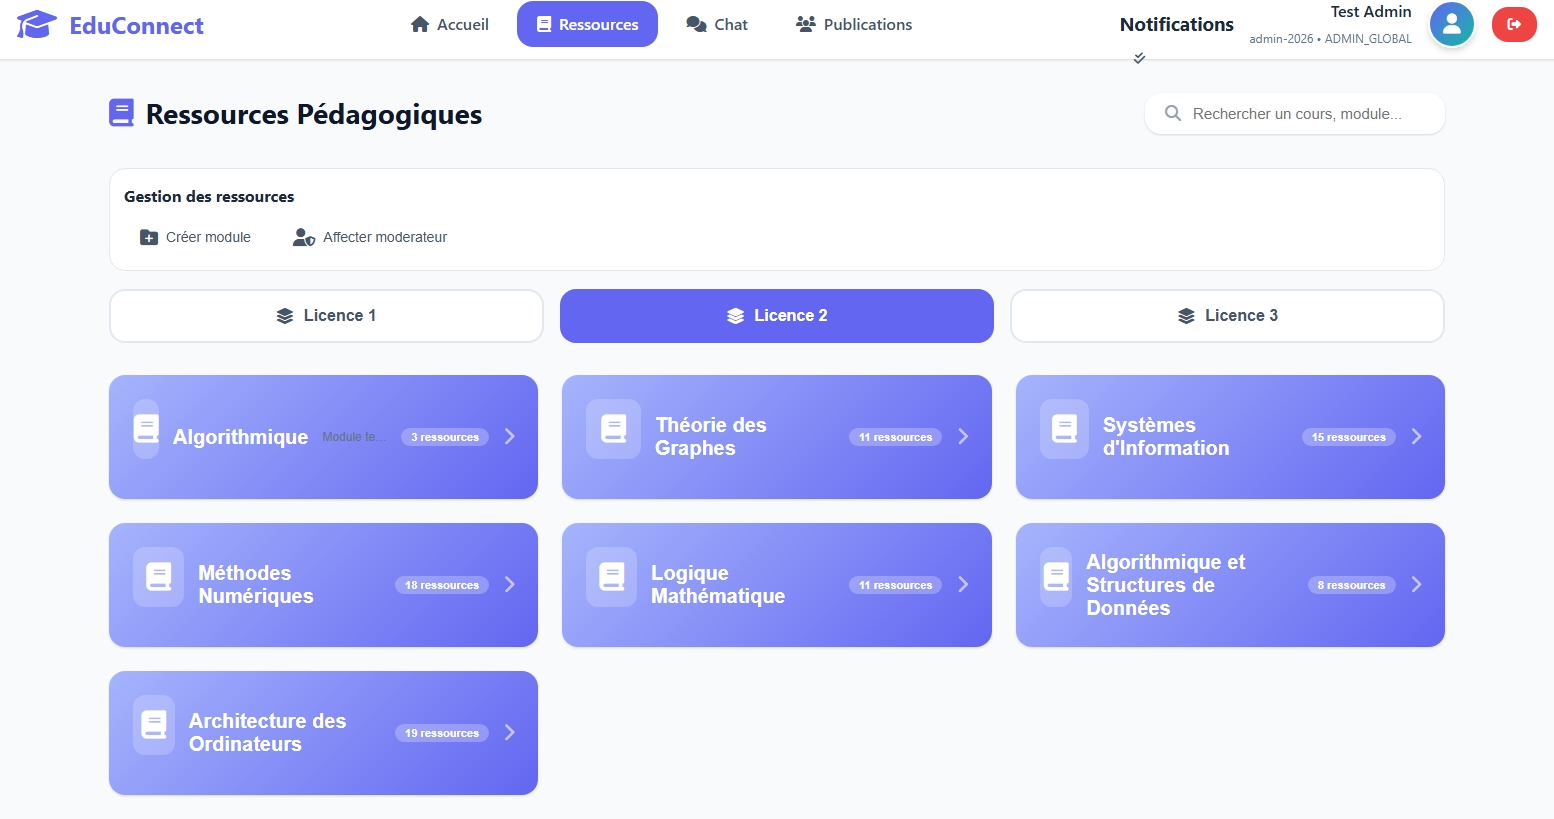
\includegraphics[width=0.85\textwidth]{figures/F1_interface_modules.png}
  \caption{Interface principale d'EduConnect~: navigation par modules (vue liste des modules par niveau).}
  \label{fig:F1}
\end{figure}

%%──────────────────────────
\subsection{Figure~2~---~Capture~: ressources dans un module}

\begin{figurebox}{Figure~2~---~Capture de la page d'un module}
\textbf{Ce que vous devez capturer~:} Une page module avec ses ressources list\'ees par section.

\textbf{Proc\'edure~:}
\begin{enumerate}
  \item Depuis la page des modules, cliquer sur un module existant (ex.~: Algorithmique, R\'eseaux, SGBD).
  \item La page d\'edi\'ee s'affiche avec les sections~: Cours, TD, TP, Examen, Corrig\'e.
  \item Les boutons \textit{Modifier} (bleu) et \textit{Supprimer} (rouge) sont visibles en vue admin~: \textbf{les montrer}.
  \item Capturer en plein \'ecran.
  \item Enregistrer sous~: \texttt{figures/F2\_interface\_ressources.png}
\end{enumerate}
\textbf{Objectif~:} D\'emontrer l'organisation hi\'erarchique Niveau\,$\to$\,Module\,$\to$\,Section\,$\to$\,Ressource avec la gestion CRUD visible.
\end{figurebox}

\begin{figure}[H]
  \centering
  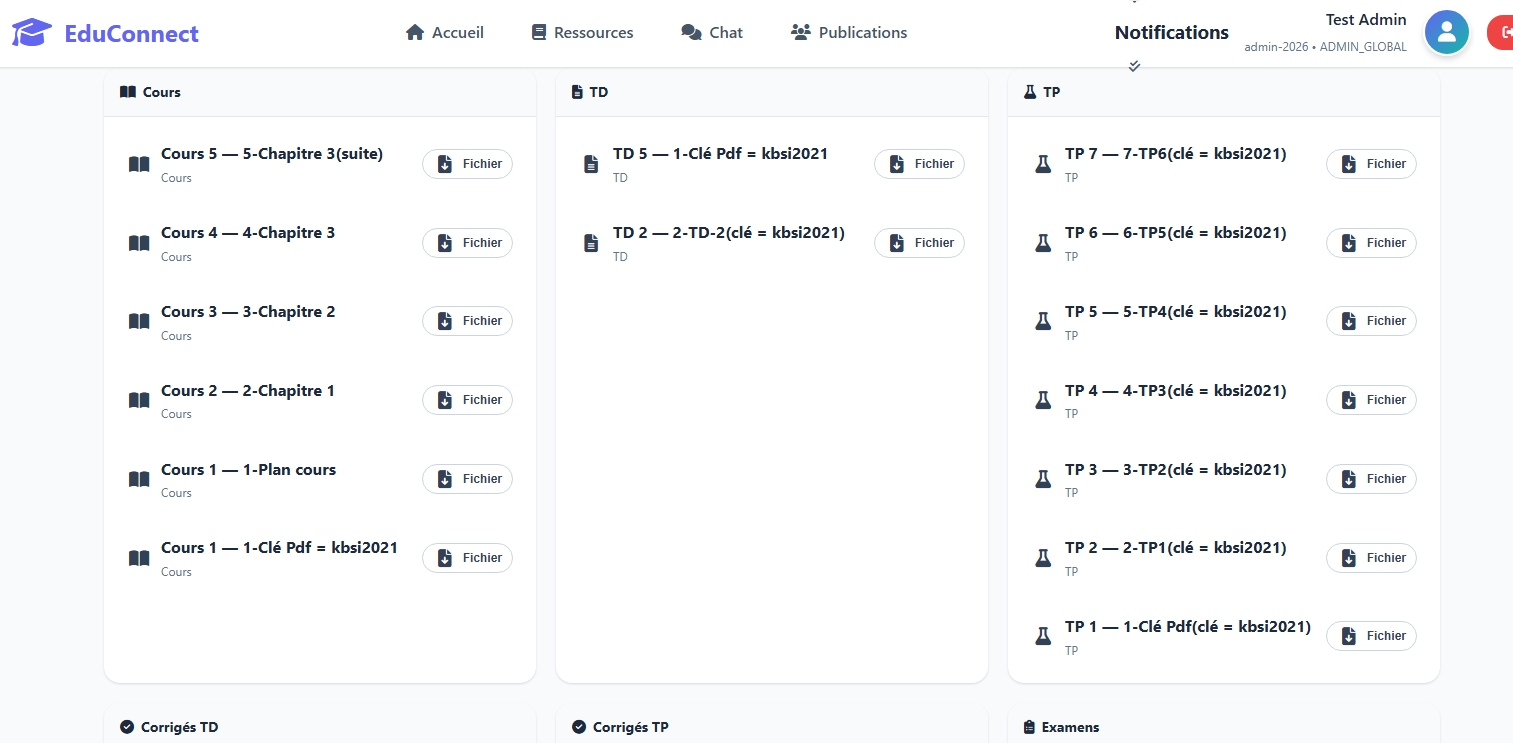
\includegraphics[width=0.85\textwidth]{figures/F2_interface_ressources.png}
  \caption{Interface d'EduConnect~: page d\'edi\'ee d'un module avec ses ressources organis\'ees par section (vue administrateur).}
  \label{fig:F2}
\end{figure}

%%──────────────────────────
\subsection{Figure~3~---~Capture~: publications et chat}

\begin{figurebox}{Figure~3~---~Capture de la couche sociale}
\textbf{Ce que vous devez capturer~:} Le fil de publications et/ou le chat.

\textbf{Proc\'edure~:}
\begin{enumerate}
  \item Cliquer sur \og{}Publications\fg{} dans le menu principal.
  \item Si vide, cr\'eer une publication de test avec quelques commentaires.
  \item Capturer le fil avec au moins une publication visible (titre, contenu, votes, commentaires).
  \item Pour le chat~: ouvrir la messagerie, ouvrir une conversation, capturer.
  \item Enregistrer sous~: \texttt{figures/F3\_interface\_social.png}
\end{enumerate}
\textbf{Objectif~:} D\'emontrer la dimension collaborative d'EduConnect absente de la majorit\'e des LMS classiques.
\end{figurebox}

\begin{figure}[H]
  \centering
  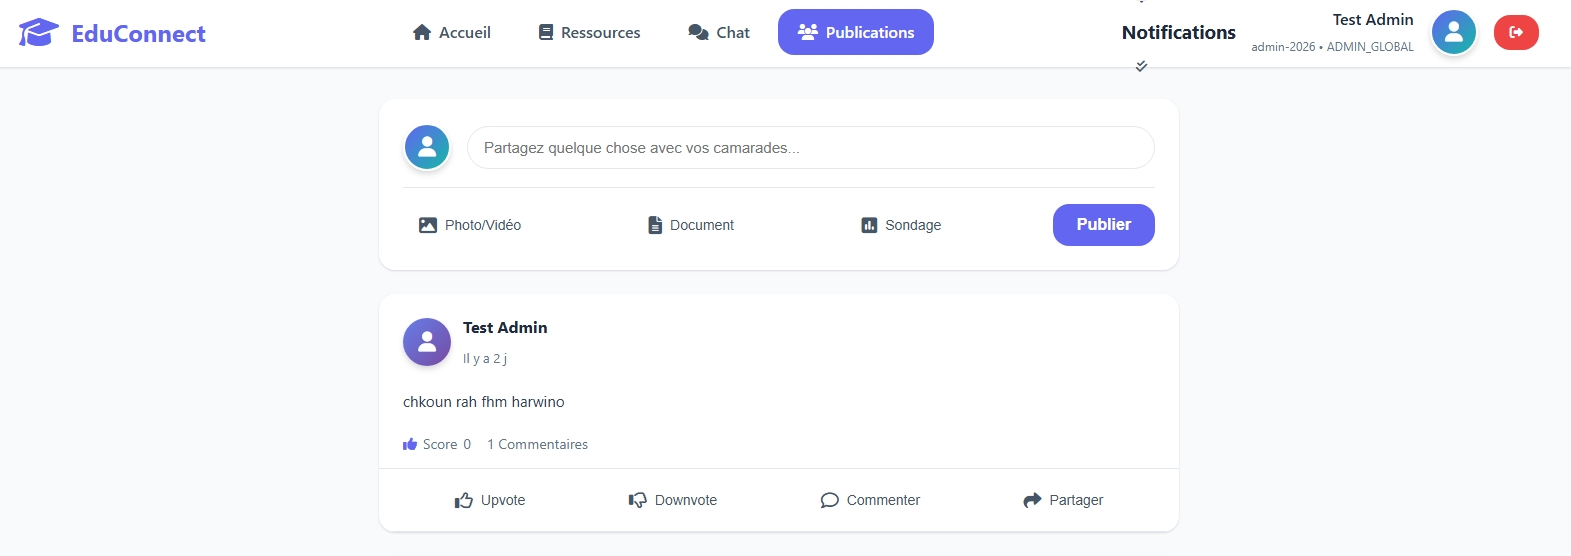
\includegraphics[width=0.85\textwidth]{figures/F3_interface_social.png}
  \caption{Interface d'EduConnect~: fil de publications et chat int\'egr\'es~--- couche sociale de la plateforme.}
  \label{fig:F3}
\end{figure}

%%──────────────────────────────────────────────────────────────────────────────
\section{Conclusion du chapitre}
\label{sec:conclusion}
%%──────────────────────────────────────────────────────────────────────────────

Ce premier chapitre a \'etabli le cadre analytique et conceptuel du projet EduConnect en articulant trois niveaux de lecture compl\'ementaires~: le contexte mondial de la transformation num\'erique de l'enseignement, les besoins sp\'ecifiques du contexte acad\'emique local de l'USTO-MB, et le positionnement d'EduConnect par rapport aux solutions existantes.

L'analyse comparative men\'ee dans la section~\ref{sec:etat_art} d\'emontre qu'aucune des plateformes \'etudi\'ees~--- Moodle, Google Classroom, Microsoft Teams Education, Canvas~--- ne couvre de mani\`ere optimale l'ensemble des exigences identifi\'ees~: navigation module-first, gouvernance \`a trois r\^oles, communication int\'egr\'ee et planification hebdomadaire d\'edi\'ee. Cette convergence de lacunes justifie pleinement la conception d'EduConnect comme solution \textit{ad hoc}, d\'evelopp\'ee sp\'ecifiquement pour le contexte universitaire local.

La suite du m\'emoire approfondit successivement la conception UML (Chapitre~2), l'impl\'ementation technique (Chapitre~3) et l'\'evaluation des r\'esultats (Chapitre~4), en s'appuyant sur le cadre th\'eorique et m\'ethodologique pos\'e dans le pr\'esent chapitre.
